\chapter{The CMS Experiment at the LHC}
\label{chapter:three}
\section{The Large Hadron Collider}

The Large Hadron Collider (LHC) is the world’s largest and most powerful particle accelerator. Inside the accelerator, two highly energetic proton beams collide up to a center-of-mass energy of 14 TeV. The LHC is constructed inside a 27 km tunnel, 100 m under the ground, located partly in Switzerland and France.

At the LHC two energetic proton beams travel in opposite directions in separate beam pipes. The proton beams travel in bunches separated by 25 ns in time. The beams travel at relativistic speeds and collide at four major interaction points at the LHC. The LHC has four main detector experiments at each interaction point: ALICE (A Large Ion Collider Experiment), ATLAS (A Toroidal LHC Apparatus), CMS (Compact Muon Solenoid), and LHCb (Large Hadron Collider beauty). ATLAS and CMS are general purpose-detectors with broad physics objectives ranging from studying the Standard Model to searching Beyond Standard Model (BSM) physics such as Dark Matter. While ALICE and LHCb are more physics dedicated detectors, ALICE and LHCb are dedicated to heavy-ion physics and studying b-quark physics respectively.

%\begin{quotation}
%    \noindent Here is a block quotation---a passage from a text you found insightful and wanted to share with others. Maybe it is from a %journal article, website, or book. Irrespective, it should support the argument being made.\footnote{A citation for the quoted material.}
%\end{quotation}

%Check appendix \ref{appendix: chapter3}

%Maybe a sentence or two that bring the argument and evidence together.\citep{dos_santos_2020}



\section{The Compact Muon Solenoid Experiment}
\subsection{Introduction}
The Compact Muon Solenoid (CMS) is a general purpose detector located in eastern France at the Large Hadron Collider (LHC) tunnel 100 m underground. It is a general purpose detector because of its broad physics searches ranging from studying the Standard Model (SM) to searching for particles that could potentially make Dark Matter (DM). CMS is a cylindrical shaped detector with 21 m in length and 15 m in cross-sectional diameter. The three main characteristics of the CMS experiment are its compactness, accurate detection of Muon particles in the muon system and its magnetic solenoid. The superconducting magnetic solenoid at the core of the CMS detector produces a continuous magnetic field of 3.8 T which is of the order of O(5) of Earth's magnetic field (0.25 - 0.65 gaus). Such large magnetic field is required for a precise measurement of the momentum of high-energy charged particles. All CMS detector subsystems are enclosed by the magnetic solenoid, the muon system, on the other hand, is on the outside. Muons are the particles that are directly detected by the CMS, with a special property that they neither stop nor decay within the boundaries of the detector. They undergo very little energy loss and thus act as a powerful medium to study high-energy process in the presence of high background.
The CMS detector is cylindrical shaped with an onion like structure, having several concentric layers of subsystems. These subsystems help prepare "photographic images" of each collision event by determining the properties of the particles in the collision. CMS has the following basic subsystems ordered from innermost to outermost:

\begin{enumerate}
    \item Silicon Tracker
    \item Electromagnetic Calorimeter
    \item Hadronic Calorimeter
    \item Superconducting Solenoid Magnet
    \item Muon System
    
    
\end{enumerate}
The CMS detector can detect 5 general categories of particles as shown in the figure below:
 \begin{enumerate}
    \item Electrons
    \item Photons
    \item Charged Hadrons
    \item Neutral Hadrons
    \item Muons
\end{enumerate}

\begin{figure} [ht]
\centering
         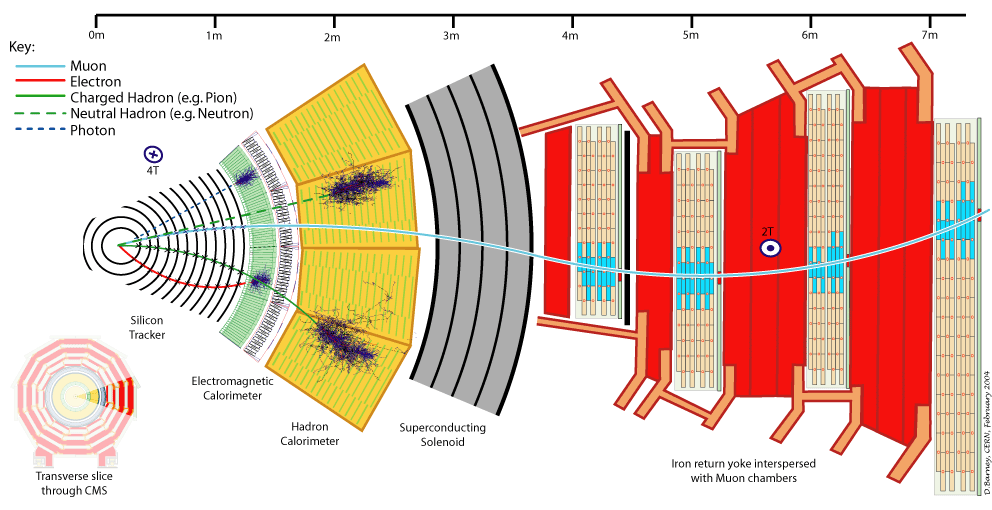
\includegraphics[width=0.9\textwidth,clip=]{thesis_template_cua/Figures/CMS_LHC_chapter/CMSSlice.png}
         \caption[#CMS Slice]{This Figure shows the cross-sectional slice of the CMS detector. Here we have shown the different sub-systems of CMS, trajectories and energy deposits of the 5 general categories of particles detected by CMS by one or more of its sub-systems}
         \label{cms_slice}
\end{figure}
%More ideas that really make this a great paper. Maybe a footnote or two.\footnote{Some peripheral thoughts that belong in a note.}
\subsection{Coordinate System}


\subsection{Silicon Tracker}

\subsection{Electromagnetic Calorimeter}

\subsection{Hadronic Calorimeter}

\subsection{Solenoid Magnet}

\subsection{Muon System}

\subsubsection{DT}

\subsubsection{RPC}

\subsubsection{CSC}

\subsection{Trigger System}